\documentclass[11pt,a4paper]{article}
\usepackage{termpaper}
\usepackage[utf8]{inputenc}
\usepackage{graphicx}
\usepackage{textcomp}
\usepackage{caption}
\usepackage{wrapfig}

%opening
\title{Boundary Labeling for annotated documents}%Vielleicht genauerer Titel?
\author{
 \authorname{Jakob Klinger} \\
 \studentnumber{1125755} \\
 \curriculum{033 534} \\
 \email{e1125755@student.tuwien.ac.at}
}

\begin{document}

\maketitle

%TODO: Abstract: \begin{abstract}...\end{abstract}

\section{Introduction}
Annotating a document is usually solved by adding footnotes or figures in an appropriate position and adding a simple reference in the text, leaving the reader to find the referenced content by themselves. Sometimes however, if a more obvious connection between the text and the referenced content is required, the reference is visibly connected to the text by drawing a straight line or a more complex path between them.

In this paper, we will look at ways to use Boundary Labeling, which means that all annotations will be placed outside of the text they are referencing and will be visually connected to the feature they are referencing. (See also \cite{Bekos2007}) While there are many papers discussing Boundary Labeling in general, only very few exist that apply this concept to written text. As a result, and since it is very easy to accidentally obscure parts of the text, this approach isn't used very often, and tends to use simplistic algorithms which produce mediocre results.
However, the papers that do discuss boundary labeling in text offer interesting contributions.

For example, the paper about the Luatodonotes-Package\cite{Kindermann2014} illustrates some of the different styles of drawing these connecting paths, and came to the conclusion that paths without bends are easier to follow. %Bild einfügen?
However, most solutions proposed in that paper don't care whether a path overlapped with text or not, which results in a decrease in readability.

The paper by Loose\cite{Loose2015} on the other hand is based around only using the free space between lines and words, which produces longer paths, and forces curves, but doesn't obscure any part of the text.
%Siehe auhc andere Papers - Motivation! (Warum will ich mir dieses Thema ansehen)


%TODO: Bezug auf Programm & Ergebnisse nehmen!

\section{Boundary Labeling} %Evtl in Introduction eingliedern?
Boundary Labeling can be explained very quickly -  connect a Point of Interest with a box containing further information which is located outside of the main area. To easily reference important concepts, some additional Terminology will be introduced (See Fig.~\ref{fig:term} for a visual explanation)

\begin{wrapfigure}{r}{0.35\textwidth}
 \captionsetup{justification=centering, margin=0.75cm}
 \raggedleft
  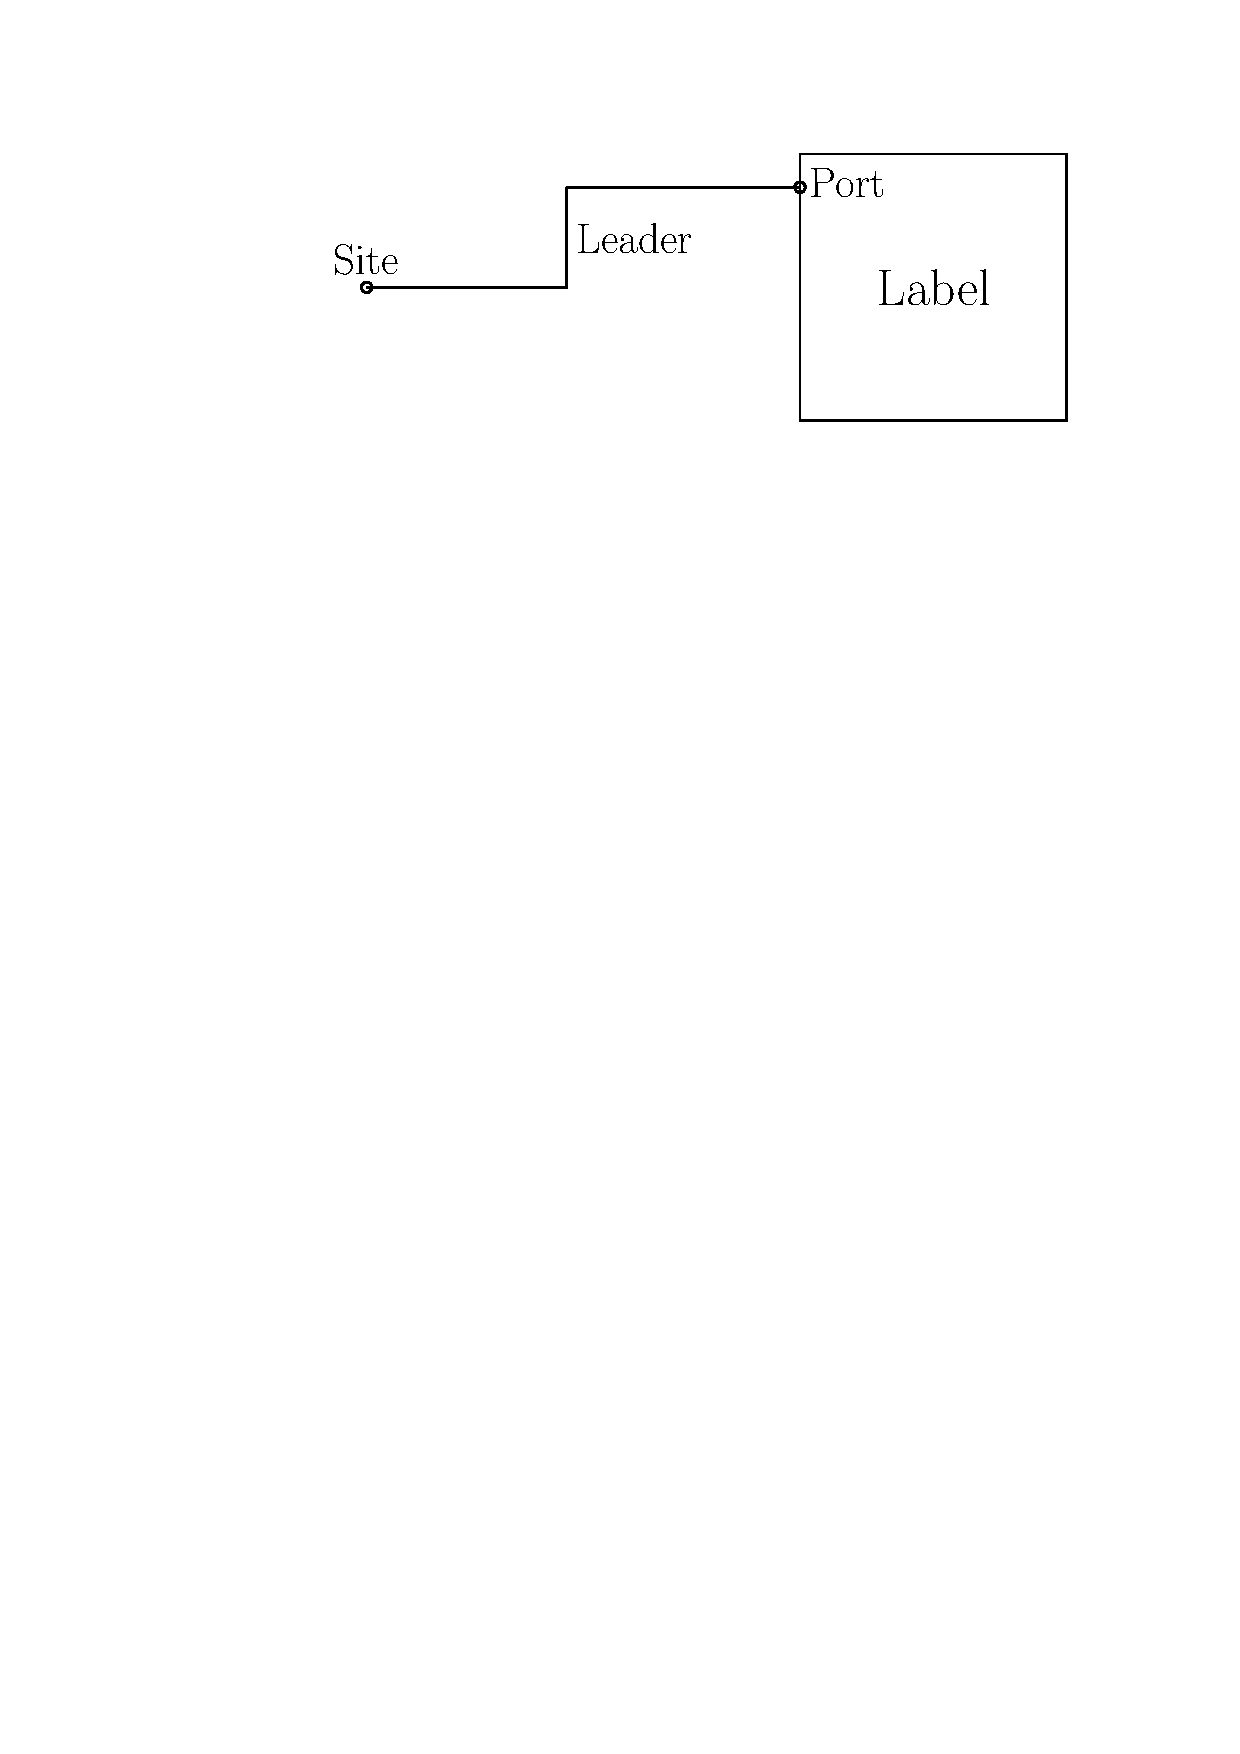
\includegraphics[scale=0.5]{IPE_TerminologyDrawing.pdf}
  \caption{Illustrated guide to the labeling terminology}
 \label{fig:term}
\end{wrapfigure}

\begin{itemize}
 \item \textbf{Label:} The additional information, usually represented as a box containing the additional information. Will also be referred to as \textbf{``Annotation''} in this paper.
 \item \textbf{Site:} The point, object or word that is labeled - without it, there wouldn't be any labeling necessary.
 \item \textbf{Leader:} The path connecting the site to the label - depending on its shape, it can be further classified into several subgroups which can be freely combined to form new leader types:
  \begin{itemize}
   \item \textit{S-Leader:} This Leader connects site and label in a straight line.
   \item \textit{O-Leader:} This leader runs orthogonally to the border between text and label area.
   \item \textit{P-Leader:} This Leader runs parallel to the border between text and label area. It must be combined with other leader styles, as it won't reach the label area otherwise.
  \end{itemize}
    For example, the leader from Fig.~\ref{fig:term} would be classified as an opo-Leader.
 \item \textbf{Port:} The location where the leader connects to the label. It may be restricted pre-determined locations, like only at the corners.
\end{itemize}
%Def. für Graphen hinzufügen! - Bei Koordinaten: Anmerken, dass 2d-euklidische Geometrie benutzt wird!

\subsection{Boundary Labeling in Documents}
As with other labeling techniques, Boundary Labeling has guidelines on how to create an optimal labeling - the leaders should be as direct as possible, no important information should be obscured, and it should be easily discernable which Label belongs to which site. These three easily come into conflict with one another, especially when labeling documents, as the text usually is very dense and leaves little space for leaders in between, yet one shouldn't allow them to pass through the text, as this makes the text harder to read. Therefore, each implementation must come to a compromise that balances these criteria.
%Beispiele von suboptimalen Lösungen einfügen? (Bilder)


%TODO: Was genau wollen wir erreichen?


%Section Ideas: The Program/Framework (Modellerklärung), The Algorithm(s), Implementation, Evaluation, Conclusion


\bibliographystyle{plain}
\bibliography{references}

\end{document}